\chapter{Fundamentos Teóricos}
Este capítulo tiene como objetivo presentar los fundamentos teóricos sobre los cuales se sustentan los métodos empleados a lo largo del trabajo, contextualizando su elección en función del problema planteado. Dado que el objetivo principal consiste en predecir múltiples características morfológicas de estructuras óseas a partir de datos tridimensionales, se abordan distintos marcos conceptuales relevantes.

En primer lugar, se introduce el campo de ML (Sección \ref{section2:ML}), base general del enfoque seguido, para luego centrarse en el subcampo de DL (Sección \ref{section2:DL}), cuyas técnicas han demostrado gran eficacia en tareas complejas de clasificación. Dentro de este marco, se abordan aspectos como la arquitectura de redes, técnicas de regularización y entrenamiento, que son fundamentales para comprender el funcionamiento de los modelos desarrollados.

A continuación, se introduce el paradigma de clasificación multietiqueta (Sección \ref{section2:multilabel}), ya que el problema actual presenta múltiples etiquetas asociadas a una misma muestra. Esta formulación no solo refleja con mayor fidelidad la naturaleza del problema, sino que también permite aprovechar posibles correlaciones entre características, lo cual puede contribuir a obtener modelos capaces de mitigar el fuerte desbalance entre clases observado en los datos. Seguidamente, se explora el método de explicabilidad Grad-CAM (Sección \ref{section2:gradcam}), el cual resulta vital para interpretar visualmente las decisiones tomadas por los modelos. Este enfoque no solo permite validar si las predicciones de los modelos coinciden con las zonas anatómicas relevantes identificadas por expertos forenses, sino que también abre la posibilidad de descubrir nuevas regiones de interés morfológico que hasta ahora no han sido consideradas por la AF.

Debido a la naturaleza tridimensional de los datos empleados, se dedica una sección específica al DL en 3D (Sección \ref{section2:3dreps}), abordando las particularidades de este tipo de modelos y su relevancia en el contexto del problema. Y justamente por la novedad de aplicar DL a datos 3D, no existen actualmente modelos base de los que partir, por lo que es necesario generar la arquitectura del modelo así como obtener sus hiperparámetros desde cero, por lo que se incluye una sección dedicada a la Búsqueda de Arquitectura Neuronal (\textit{Neural Architecture Search}, NAS) (Sección \ref{section2:nas}). Además, estas técnicas se emplean como otra estrategia para afrontar el fuerte desbalanceo entre clases, ya que también permiten optimizar arquitecturas robustas frente a este tipo de situaciones.

En conjunto, este capítulo busca ofrecer una comprensión clara y estructurada de los pilares teóricos que sustentan las decisiones metodológicas adoptadas en este TFM, facilitando así la interpretación de los capítulos posteriores.

\section{Aprendizaje Automático}
\label{section2:ML}
El Aprendizaje Automático, o \textit{Machine Learning} (ML) \cite{abu-mostafa_learning_2012, bishop_pattern_2019, murphy_probabilistic_2022, murphy_probabilistic_2023, 6284961}, es una rama de la Inteligencia Artificial (IA) que se enfoca en el desarrollo de programas informáticos para resolver tareas complejas donde no existe una solución analítica directa. Es decir, son tareas donde no es factible diseñar un algoritmo tradicional que defina de forma explícita la transformación de los datos de entrada en los de salida, debido a su complejidad o ambigüedad. En estos casos, a menudo se carece de un conocimiento detallado y completo del problema, lo que puede intentarse compensar mediante el uso de datos relacionados. Estos datos pueden emplearse para obtener una solución empírica, donde el sistema \say{aprende} de ellos. A partir de los datos, se extraen patrones o reglas que permiten construir un algoritmo aproximado, conocido como modelo, capaz de resolver la tarea incluso cuando se enfrenta a datos no vistos previamente. Formalmente, se puede definir que un programa aprende de la experiencia $E$ en relación con una clase de tareas $T$ y una métrica de rendimiento $P$ si su rendimiento en las tareas $T$, medido por $P$, mejora con la experiencia $E$. Este aprendizaje se clasifica en dos grandes grupos: supervisado y no supervisado. En el aprendizaje supervisado, se dispone tanto de los datos de entrada como de las salidas correctas correspondientes, mientras que en el aprendizaje no supervisado solo se tienen los datos de entrada y se espera que el programa identifique patrones dentro de estos.

En términos generales, es factible aplicar ML en problemas que cumplen con alguna de las siguientes condiciones: (a) cuando se dispone de extensas bases de datos que permiten extraer patrones intrínsecos, lo que se conoce como minería de datos o \textit{data mining} \cite{alma991006986149704990}; (b) en aquellos problemas cuyos dominios no están bien definidos o en los que resulta difícil para un humano describirlos de manera precisa para desarrollar un algoritmo, como ocurre en tareas de detección de objetos en imágenes; y (c) en dominios en los que el sistema debe adaptarse de forma dinámica a condiciones cambiantes \cite{murphy_probabilistic_2023}.

En el aprendizaje supervisado se distinguen dos tareas fundamentales: la clasificación y la regresión, cuya principal diferencia radica en la naturaleza de la variable de salida. En las tareas de clasificación, cada ejemplo de entrada se asigna a una categoría discreta. Esto implica que el modelo debe aprender a identificar y etiquetar cada muestra dentro de un conjunto finito de clases. Por otro lado, en las tareas de regresión el objetivo es predecir un valor numérico continuo. En este caso, la salida del modelo puede tomar cualquier valor dentro de un rango determinado.

A partir de las descripciones previas, se puede concluir que es viable aplicar técnicas de ML al problema en cuestión. En este caso, se dispone de datos de entrada, que corresponden a los huesos de la sínfisis del pubis, y de datos de salida, representados por los atributos de cada hueso clasificados según las nueve categorías del método de Todd. Además, aunque los antropólogos forenses poseen el conocimiento experto necesario para identificar estos patrones, dicho conocimiento no puede expresarse de manera analítica. Por ello, el problema se enmarca dentro del aprendizaje supervisado, siendo específicamente un problema de clasificación, ya que es necesario asignar a cada hueso los atributos correspondientes a las categorías establecidas por el método de Todd.

\section{Aprendizaje Profundo}
\label{section2:DL}
El aprendizaje profundo (\textit{Deep Learning}, DL) \cite{Goodfellow-et-al-2016, bishop_deep_2024, prince_understanding_2023, lecun_deep_2015, schmidhuber_deep_2015} es una subdisciplina de ML en la que el modelo se encarga de aprender y extraer de manera automática las características relevantes a partir de los datos del problema. Esta aproximación contrasta con otras técnicas de ML en las que las características son diseñadas manualmente o \textit{handcrafted} por expertos que utilizan su conocimiento específico del dominio. Se ha demostrado que, para problemas de alta complejidad, las características extraídas de forma automática tienden a ser más efectivas y eficientes en comparación con aquellas obtenidas manualmente.

El modelo predominante en el ámbito del DL es la red neuronal artificial (\textit{Artificial Neural Network}, ANN) \cite{bishop_ANN, ripley_ANN}, compuesta por nodos de procesamiento, denominados \say{neuronas}{\interfootnotelinepenalty=10000 \footnote{Aunque su denominación es bioinspirada en la corteza visual del cerebro, estos modelos no simulan de forma precisa el funcionamiento biológico neuronal.}}, interconectados en diferentes capas. La red se estructura con una capa de entrada, que recibe los datos en bruto, seguida de una o varias capas ocultas encargadas de aprender y extraer progresivamente las características relevantes, y una capa de salida. En las capas iniciales se capturan atributos de bajo nivel, mientras que las subsiguientes permiten obtener representaciones más abstractas y de alto nivel, facilitando la solución del problema planteado. La cantidad de capas en una ANN define su profundidad, lo que justifica el término aprendizaje profundo: en general, a mayor número de capas, se logra un aprendizaje más detallado y eficaz. Un ejemplo clásico de una ANN se ilustra en la Figura \ref{fig:annExample}, donde se diferencia entre una red superficial y una red profunda.

\begin{figure}[h]
    \centering
    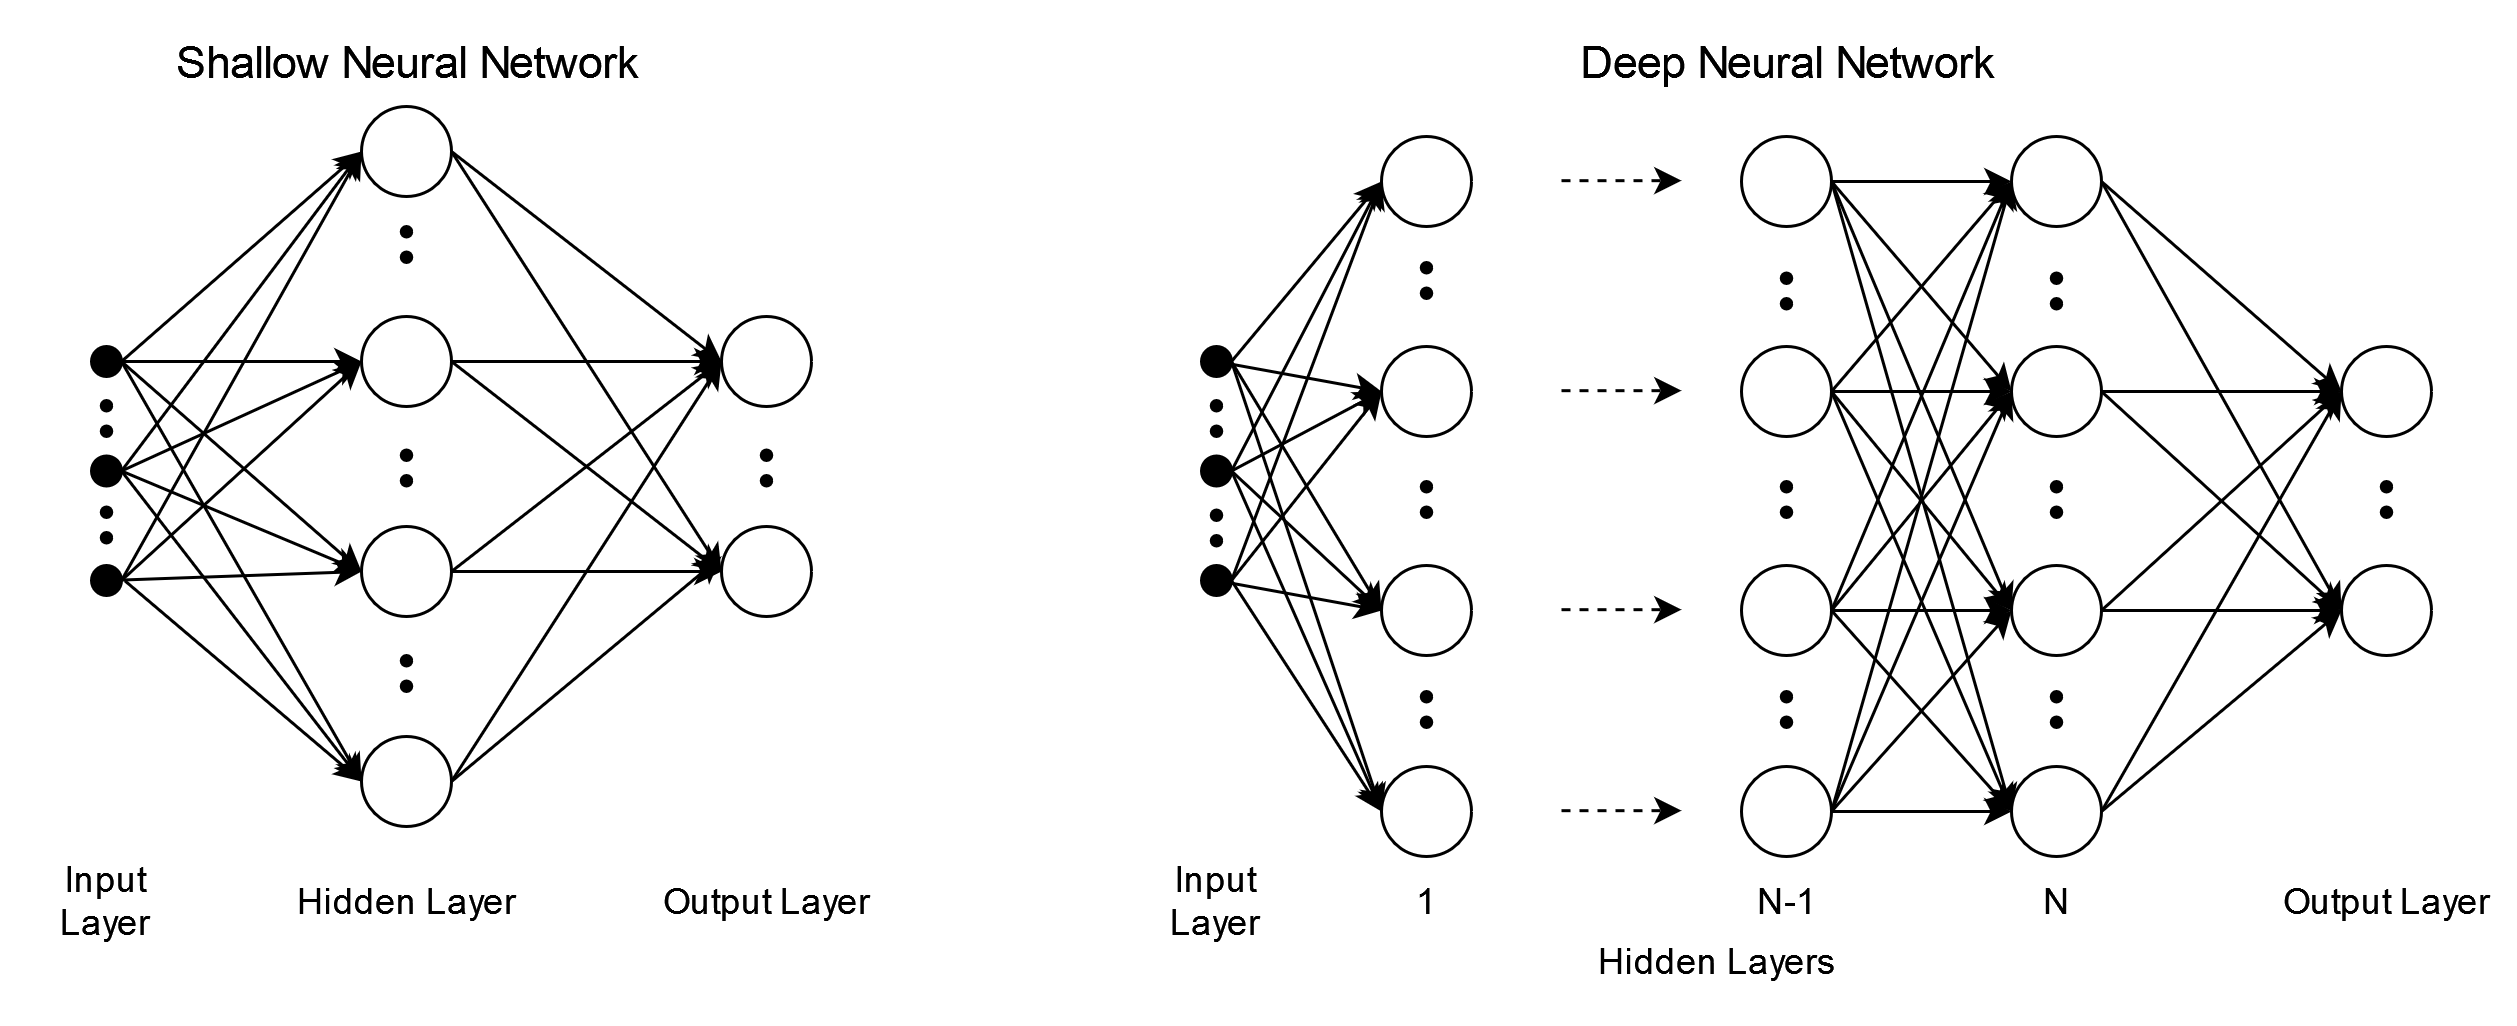
\includegraphics[width=\linewidth]{figures/2_theory/neuralNetDiagram.png}
    \caption[Ejemplos de la estructura de una ANN]{Ejemplos típicos de la estructura de una ANN, en este caso se tiene una red superficial o \textit{shallow} a la izquierda con una sola capa oculta entre las capas de entrada y salida; y una red profunda o \textit{deep} a la derecha, que posee múltiples capas con variable densidad de neuronas entre las capas de entrada y salida. Figura tomada de \cite{annPictureSource}.}
    \label{fig:annExample}
\end{figure}

Cada neurona, como se ha descrito, recibe múltiples valores de entrada y produce un valor de salida que sirve como entrada para la siguiente capa. Además, cada neurona incorpora una función de activación no lineal, la cual transforma las entradas en el valor de salida que se transmite. Esta función actúa de manera similar a un umbral, permitiendo que la red amplifique ciertas señales y suprima otras, en función de lo que se desea aprender. Dicho comportamiento se logra mediante la asignación de pesos a cada entrada de la neurona, junto con un valor adicional conocido como sesgo o \textit{bias}. La modificación de los pesos y el sesgo permite ajustar la magnitud de la señal procesada por la función de activación. Un ejemplo visual de una neurona artificial se puede observar en la Figura \ref{fig:artificialNeuronExample}.

\begin{figure}[h]
    \centering
    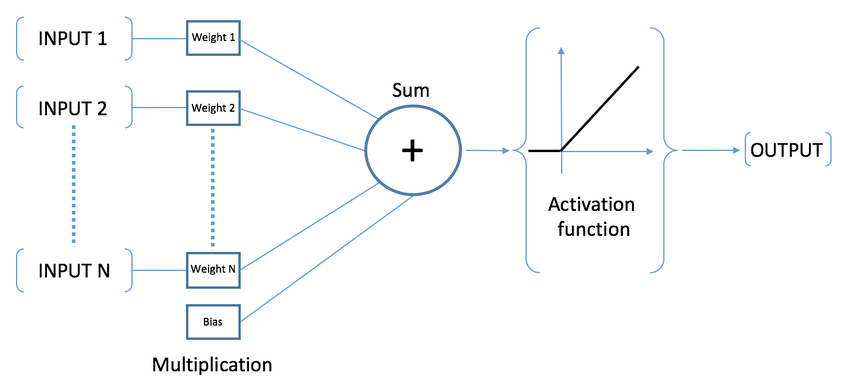
\includegraphics[width=\linewidth]{figures/2_theory/artificialNeuron.png}
    \caption[Ejemplo de una neurona artificial]{Ejemplo de una neurona artificial, los datos de entrada son multiplicados por los pesos y su resultado, junto con el sesgo (o \textit{bias}), son combinados linealmente. A continuación, son transformados por la función no lineal o de activación para proporcionar el valor salida de la neurona. Figura tomada de \cite{artificialNeuron}.}
    \label{fig:artificialNeuronExample}
\end{figure}

El aprendizaje en una ANN consiste esencialmente en ajustar los pesos y el sesgo de cada neurona para que, tras ser procesados por la función de activación, se puedan extraer y transformar las características más relevantes de los datos. El proceso inicia con la propagación hacia adelante (\textit{forward propagation}), en la cual los datos atraviesan la red desde la capa de entrada, pasando por las capas ocultas, hasta llegar a la capa de salida. Durante esta fase, se calculan los valores de salida de cada neurona, lo que finalmente permite obtener un resultado global de la red.

En este punto entra en juego la función de pérdida o error, cuya finalidad es medir qué tan bien ha aprendido la red. Existen diversas funciones de pérdida, y la elección de una en particular depende del tipo de problema y del enfoque de aprendizaje utilizado. A partir del valor de error obtenido, se aplica el algoritmo de retropropagación (\textit{backpropagation}), el cual calcula las derivadas de los pesos y sesgos respecto a dicho error. Posteriormente, mediante el uso de un algoritmo de optimización (\textit{optimizer}), se recalculan los valores de los pesos con el objetivo de minimizar el error de manera iterativa.

Este procedimiento, conocido como entrenamiento, permite que la red ajuste sus parámetros de manera progresiva hasta alcanzar un modelo que represente de manera óptima los patrones de los datos. Sin embargo, este enfoque de aprendizaje presenta un desafío fundamental en ML: el sobreentrenamiento u \textit{overfitting}. Este fenómeno ocurre cuando el modelo se ajusta excesivamente a los datos de entrenamiento, perdiendo capacidad de generalización. En tales casos, la red logra un error muy bajo en el conjunto de entrenamiento, pero su desempeño se deteriora considerablemente cuando se enfrenta a datos nuevos o no vistos previamente.

\subsection{Redes Neuronales Convolucionales}
\label{section2:cnn}
Las redes neuronales convolucionales (\textit{Convolutional Neural Network}, CNN) \cite{lecun_backpropagation_1989, leCUM_CNN} son un tipo de red neuronal artificial ampliamente utilizada en tareas de procesamiento, clasificación y segmentación de imágenes. Además, su aplicación se ha extendido a otras áreas como el procesamiento de texto, sonidos y, más recientemente, el análisis de superficies tridimensionales. A diferencia de una ANN tradicional, en la que todas las neuronas están completamente conectadas entre sí, una CNN introduce dos tipos adicionales de capas: capas convolucionales y capas de \textit{pooling}.

La estructura básica de una CNN puede visualizarse en la Figura \ref{fig:cnnExample}, donde se observa que la red está dividida en dos partes fundamentales. La primera parte está compuesta exclusivamente por capas convolucionales y de \textit{pooling}, cuyo propósito es extraer características relevantes de los datos de entrada. En la segunda parte, la estructura se asemeja a una ANN clásica, en la que las características extraídas se combinan de manera no lineal, permitiendo que la red realice tareas como la clasificación o detección de patrones dentro de los datos procesados.

\begin{figure}[h]
    \centering
    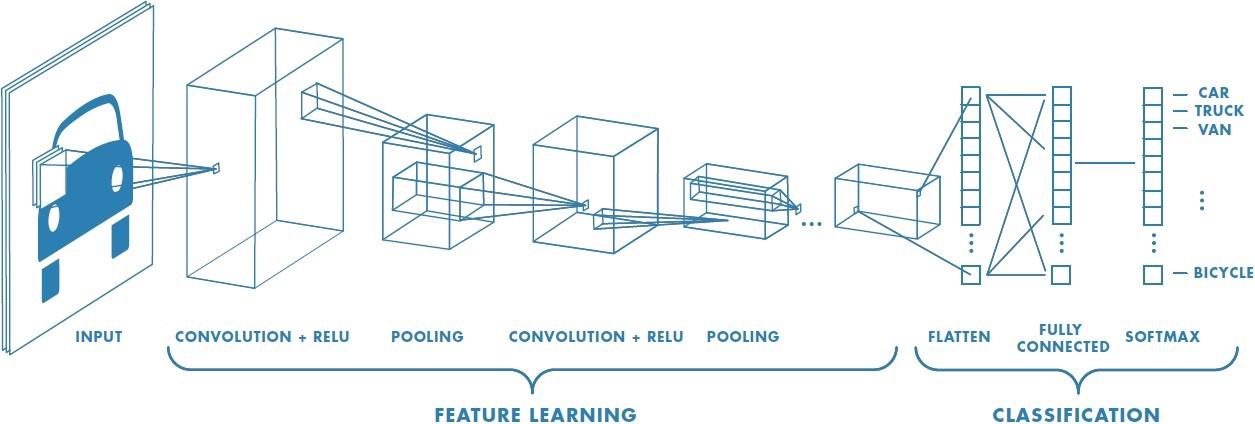
\includegraphics[width=\linewidth]{figures/2_theory/cnnExample.jpeg}
    \caption[Estructura básica de una CNN]{Estructura básica de una CNN, en la que se aprecia su organización típica: una serie de capas convolucionales con funciones de activación no lineales, intercaladas con capas de \textit{pooling}, que conforman la etapa inicial de extracción de características (\textit{Feature Learning} en la imagen). Esta parte es seguida por una serie de capas totalmente conectadas que conducen hasta la capa de salida. En este ejemplo, la red aborda un problema de clasificación. Figura tomada de \cite{prabhu_understanding_2019}.}
    \label{fig:cnnExample}
\end{figure}

\subsection{Capa convolucional}
La capa convolucional es el elemento central de una CNN. A diferencia de una ANN clásica, en la que cada neurona está conectada con todas las neuronas de las capas vecinas, en una capa convolucional cada neurona está conectada únicamente a un vecindario local de neuronas. Esto es posible gracias a la operación de convolución, la cual permite procesar la imagen de entrada de manera eficiente\footnote{De aquí en adelante, se explicará el funcionamiento de la CNN clásica aplicada a imágenes, aunque su principio es similar en otros tipos de datos.}.

Una convolución consiste en un producto punto entre dos matrices:
\begin{itemize}
    \item El \textit{kernel} (filtro o núcleo de la convolución), que es un conjunto de pesos que la red puede aprender y modificar.
    \item El campo receptivo (\textit{receptive field}), que es un fragmento de la imagen con el que el \textit{kernel} se multiplica en un momento dado.
\end{itemize}

El \textit{kernel} se desplaza por la imagen, comenzando en una esquina y moviéndose a través de filas y columnas de píxeles hasta recorrer toda la imagen. La matriz resultante de esta operación se procesa mediante una función no lineal, al igual que en una neurona clásica, y genera un mapa de características o mapa de activación, que servirá como entrada para la siguiente capa de la red.

Gracias a este proceso, la CNN puede capturar patrones espaciales y temporales en los datos mediante la aplicación de filtros relevantes. En las primeras capas convolucionales, la red aprende características de bajo nivel (como bordes y texturas), que luego se combinan en las capas siguientes para identificar características de alto nivel (como formas y estructuras más complejas).

Sin embargo, la aplicación directa de la convolución sobre una imagen reduce el tamaño del mapa de activación debido a la propia naturaleza del operador. Para mitigar esto, se pueden emplear técnicas como:
\begin{itemize}
    \item Relleno (\textit{padding}): Se añaden píxeles alrededor de la imagen utilizando información ya presente en ella, lo que permite mantener la misma dimensionalidad en la salida.
    \item Saltos (\textit{strides}): Se modifica el número de píxeles que avanza el kernel en cada paso, lo que puede reducir aún más la salida de la capa convolucional.
\end{itemize}

\subsection{Capa de \textit{pooling}}

Las capas de \textit{pooling} tienen como único objetivo reducir la dimensionalidad del mapa de activación generado por las capas convolucionales. Por ello, se insertan inmediatamente después de estas. Aunque las propias convoluciones pueden disminuir la resolución de los mapas de activación, el \textit{pooling} ofrece una forma más controlada de lograrlo y, además, mejora la extracción de características.

El \textit{pooling}, al igual que la convolución, utiliza un filtro o ventana que se desplaza a lo largo de los datos con un determinado salto (\textit{stride}). Sin embargo, en lugar de aplicar una operación de convolución, se realizan operaciones de reducción, como:
\begin{itemize}
    \item \textit{Max Pooling}: Se selecciona el valor máximo dentro de la ventana, lo que ayuda a preservar las características más relevantes y genera mayor invarianza a la traslación.
    \item \textit{Average Pooling}: Se calcula el promedio de los valores dentro de la ventana, lo que suaviza la salida y reduce el ruido en los datos.
\end{itemize}

Las capas convolucionales y de \textit{pooling} en conjunto conforman la sección de extracción de características en una CNN. Dependiendo de la complejidad del problema, el número de estas capas puede variarse para asegurar que la red extraiga las características esenciales necesarias para el aprendizaje.

\subsection{Capa totalmente conectada}
Las capas totalmente conectadas o densas (\textit{fully connected} o \textit{dense layers}) aparecen después de las capas de convolución y \textit{pooling}, y constituyen la parte final de una CNN. Estas capas siguen la estructura de una ANN clásica, donde cada neurona está conectada con todas las neuronas de las capas adyacentes. Tomando como entrada las características extraídas y de ellas aprenden combinaciones no lineales. Gracias a esto, la red neuronal puede cumplir su objetivo, ya sea la clasificación o la regresión.

La última capa densa es la salida de toda la red. En esta etapa, se evalúa la función de pérdida, que mide la diferencia entre la predicción del modelo y la realidad. Luego, mediante \textit{backpropagation} y un algoritmo de optimización, los pesos de todas las neuronas de la red se ajustan durante el entrenamiento para minimizar el error.

\subsection{Regularización}
\label{subsection:regularization}
La regularización engloba un conjunto de técnicas destinadas a mitigar el problema del sobreajuste u \textit{overfitting}. Una dificultad que, como ya se ha comentado, es frecuente en ANNs y CNNs. Consisten en modificaciones que buscan mejorar la capacidad de generalización del modelo, ya sea limitando su complejidad, restringiendo sus parámetros o ajustando el comportamiento de la red \cite{Goodfellow-et-al-2016}. En el contexto de este proyecto, las estrategias de regularización más relevantes son: la normalización, el uso de la detención anticipada (\textit{Early Stopping}) y la inicialización de los pesos de la red.

\subsubsection{Normalización}

\begin{figure}[h]
    \centering
    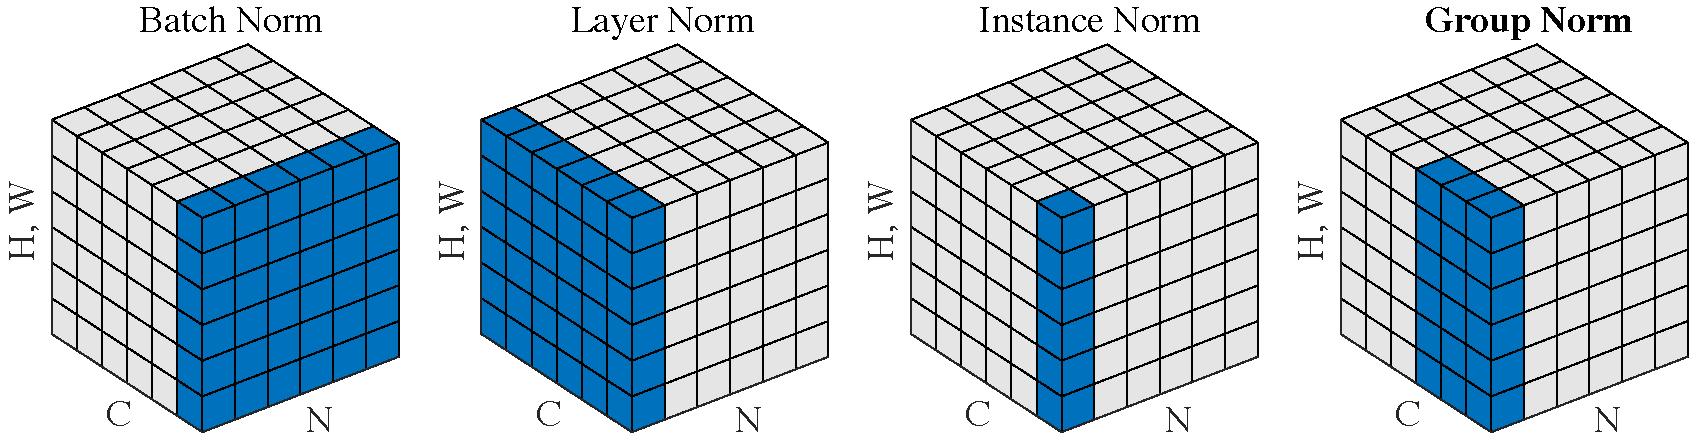
\includegraphics[width=\linewidth]{figures/2_theory/normTypes.pdf}
    \caption[Tipos de normalización]{Tipos de normalización. Cada subgráfico muestra un tensor de mapa de características, donde N representa el eje del lote (\textit{batch}), C el eje de los canales, y (H, W) los ejes espaciales. Los píxeles en azul se normalizan utilizando la misma media y varianza, calculadas agregando los valores de dichos píxeles. Figura tomada de \cite{wu2018group}.}
    \label{fig:normTypes}
\end{figure}


La normalización es una técnica que estandariza los datos de manera que el valor medio de los mismos sea cercano a 0, con una desviación estándar cercana a 1. Empíricamente se ha demostrado que esto mejora el rendimiento de las redes, pues evita que los pesos posean valores muy grandes, lo que afecta el cálculo de gradientes \cite{ioffe_batch_2015}. 

Por lo general la normalización se aplica a las capas convolucionales de la red y la manera típica de utilizarla es haciendo uso de la normalización por lotes o \textit{batch normalization}, en donde se aplica la estandarización a una característica $i$-ésima de entrada calculando la media y desviación típica de todas las características $i$-ésimas del lote. Existe también la normalización por capa o \textit{layer normalization} que aplica la media y desviación típica por cada capa independiente del lote, la normalización por instancia o \textit{instance normalization} que normaliza cada canal por separado. Por último se tiene la normalización por grupo o \textit{group normalization} que aplica la normalización a un grupo de canales pero no toda la capa entera. El uso de un tipo u otro de normalización depende de la tarea a cumplir, pues se sabe que empíricamente diferentes tipos producen mejores modelos en diferentes problemas. Un ejemplo visual de todos los tipos de normalización mencionados se puede observar en la Figura \ref{fig:normTypes}. 

\subsubsection{\textit{Early Stopping}}
La técnica de regularización conocida como detención anticipada o \textit{Early Stopping} \cite{prechelt_early_1998} busca mitigar el \textit{overfitting} mediante el monitoreo continuo del entrenamiento. Su principio es detener el proceso de aprendizaje en el momento en que el rendimiento del modelo comienza a degradarse, lo cual suele indicar que ha empezado a memorizar los datos del conjunto de entrenamiento en lugar de generalizar. Para detectar esta degradación, se emplea un conjunto adicional de datos denominado de \say{validación}, que no interviene en el entrenamiento, pero se utiliza tras cada época para evaluar el desempeño del modelo, ya sea mediante una métrica específica o a través del error de pérdida.

La decisión de detener el entrenamiento se toma mediante una heurística, que puede consistir en alguno de los siguientes criterios: ausencia de mejora en la métrica después de un número determinado de épocas consecutivas, mejoras inferiores a un umbral mínimo, o bien la consecución de un valor objetivo predefinido. Esta técnica además permite combinarse con el llamado \textit{Model Checkpointing} \cite{geron_hands-machine_2019}, que consiste en guardar automáticamente el estado del modelo (o sus pesos) en el punto donde se obtuvo el mejor rendimiento sobre el conjunto de validación, en lugar de almacenar simplemente la última iteración del entrenamiento.

\subsubsection{Inicialización de los pesos}
La inicialización de pesos es el procedimiento mediante el cual se asignan valores iniciales a cada peso y sesgo de las neuronas que componen de una ANN o CNN. Se trata de una técnica de regularización debido a que la selección de estos valores iniciales influencia en gran manera el desempeño del modelo al ser entrenado \cite{Goodfellow-et-al-2016}.

Existen diversas maneras de obtener estos valores iniciales: La más directa es obtener valores aleatorios por medio de una distribución normal o uniforme dentro de un rango de valores. Si bien se obtienen buenos resultados por medio de esta inicialización, se ha observado que aplicando diversas heurísticas es posible mejorar más aún la calidad del aprendizaje de un modelo.

La inicialización Xavier o Glorot \cite{glorot2010understanding} es una inicialización aleatoria uniforme que toma en cuenta el número de entradas y salidas que posee cada capa para obtener los valores aleatorios de cada neurona en dicha capa, de tal forma que el rango que posee cada neurona se reduce con la raíz cuadrada del número de entradas y salidas de la capa en la que se encuentra. Existe una variante conocida como inicialización Kaiming o He \cite{he2015delving} que reemplaza la distribución uniforme por una gaussiana, acotada por las entradas que posee cada capa de la red. Por otro lado existe la inicialización Ortogonal u \textit{Orthogonal} \cite{saxe_exact_2013} que inicializa los pesos de forma aleatoria, pero con la condición de que entre cada capa los valores sean ortogonales entre sí, es decir, que al realizar la multiplicación de matrices se obtenga la matriz identidad. En general estos métodos permiten mantener estabilidad numérica y evitan que las gradientes calculadas sean demasiado grandes o pequeñas, lo que a su vez, mejora la convergencia del modelo.

\FloatBarrier

\section{Clasificación Multietiqueta}
\label{section2:multilabel}

\begin{figure}[htb]
    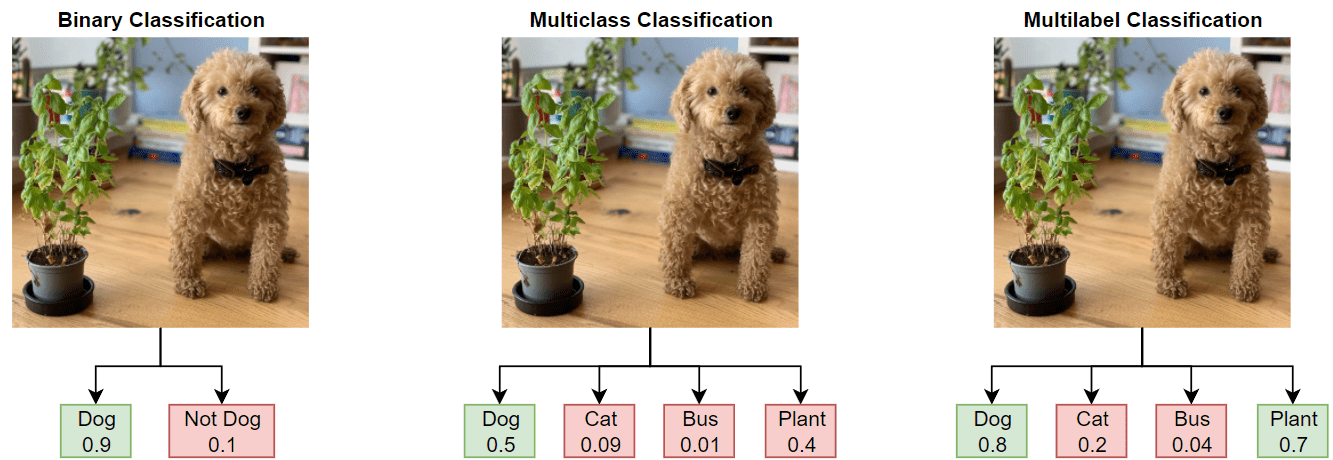
\includegraphics[width=\linewidth]{figures/2_theory/multilabel_example.png}
    \caption[Ejemplo comparativo entre clasificación binaria, multiclase y multietiqueta]{Ejemplo comparativo entre clasificación binaria, multiclase y multietiqueta. A la izquierda se muestra un clasificador binario, que determina si una única etiqueta está presente o no, en este caso si la imagen contiene un perro. En el centro, un clasificador multiclase, que asigna exactamente una clase entre varias posibles a cada muestra; aquí, la imagen es clasificada únicamente como \say{perro}, ignorando la planta. A la derecha, un clasificador multietiqueta, que permite asignar múltiples etiquetas simultáneamente a una misma entrada, reflejando mejor situaciones en las que varios atributos pueden coexistir; en este caso, se reconocen correctamente tanto el perro como la planta. Figura tomada de \cite{noauthor_multilabel_nodate}.}
    \label{multilabel_example}
\end{figure}

Como se ha descrito anteriormente, la clasificación multiclase emplea una variable de salida asociada a una variable discreta. Sin embargo, existe una extensión de esta idea en la que, para cada variable de entrada, pueden existir múltiples categorías asociadas que no se solapan entre sí. Este enfoque se conoce como clasificación multietiqueta o \textit{multi-label classification} \cite{tarekegn_deep_2024}.

En un problema de clasificación multiclase tradicional, cada instancia se asigna exclusivamente a una única clase dentro de un conjunto finito y mutuamente excluyente de categorías. Por ejemplo, en la clasificación de imágenes en redes sociales, un modelo puede etiquetar una imagen como \say{perro} o \say{planta}, pero nunca ambas simultáneamente. En cambio, en un problema de clasificación multietiqueta, una misma instancia puede estar asociada a múltiples etiquetas a la vez. Siguiendo el ejemplo anterior, una foto podría ser etiquetada simultáneamente como \say{perro} y \say{planta}, como se ilustra en la Figura \ref{multilabel_example}.

Entre los algoritmos de ML más utilizados para la clasificación multietiqueta destacan los árboles de decisión, los métodos de vecinos más próximos, las máquinas de vectores de soporte y las redes neuronales. En particular, las redes neuronales han logrado mejoras en el aprendizaje cuando se utiliza este método \cite{ranjan_hyperface_2019}.

Dado que el problema en cuestión involucra la clasificación de huesos de la sínfisis del pubis según las nueve categorías del método de Todd, es posible abordarlo mediante un enfoque de clasificación multietiqueta, donde bien se utilicen todas o algunas de las características en un único modelo de DL en vez de un modelo por cada característica.

\section{Grad-CAM}
\label{section2:gradcam}

\begin{figure}[h]  
    \centering
    \begin{subfigure}{0.28\textwidth}
        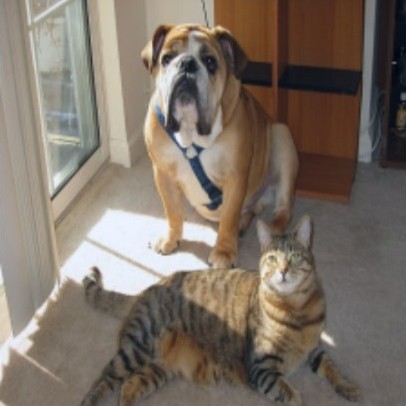
\includegraphics[width=\textwidth]{figures/2_theory/grad_cam__og.jpg}
        \begin{minipage}{.1cm}
            \vfill
            \end{minipage}
        \caption{Fotografía original.}
        \label{fig__grad_cam__og}
    \end{subfigure}
    \begin{subfigure}{0.28\textwidth}
        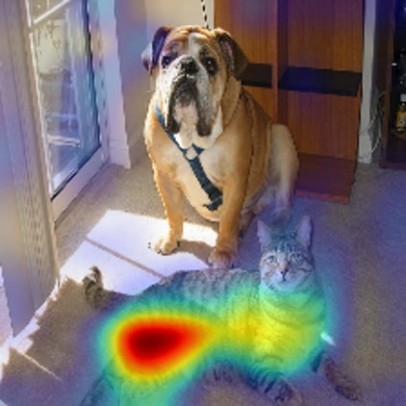
\includegraphics[width=\textwidth]{figures/2_theory/grad_cam__cat.jpg}
        \caption{Mapa de activación para la clase \say{gato}.}
        \label{fig__grad_cam__cat}
    \end{subfigure}  
    \begin{subfigure}{0.28\textwidth}
        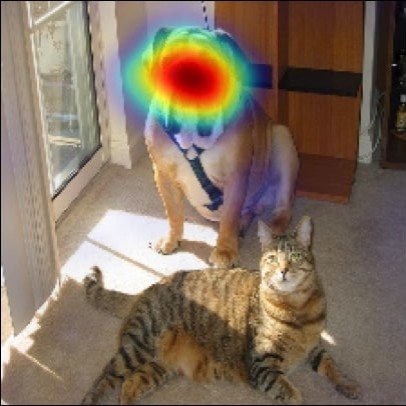
\includegraphics[width=\textwidth]{figures/2_theory/grad_cam__dog.jpg}
        \caption{Mapa de activación para la clase \say{perro}.}
        \label{fig__grad_cam__dog}
    \end{subfigure}    
    \caption[Ejemplo de funcionamiento de Grad-CAM]{Ejemplo ilustrativo del funcionamiento de Grad-CAM. A partir de la imagen original (a), si se analiza la clase \say{gato}, se obtiene el mapa de activación (b), donde se resaltan las regiones que más han contribuido a la predicción de dicha clase. Al estudiar la clase \say{perro}, se genera el mapa (c). Esta técnica proporciona una forma de explicabilidad visual sobre las decisiones tomadas por una CNN. Figura tomada de \cite{selvaraju_grad_cam_2017}.}   
    \label{fig__grad_cam}  
\end{figure}

A pesar de que las ANNs y, en particular, las técnicas de DL, han demostrado una capacidad sobresaliente para resolver una amplia variedad de tareas complejas con altos niveles de precisión, una de sus principales limitaciones radica en su carácter de \say{caja negra}. Es decir, aunque son capaces de ofrecer soluciones efectivas, comprender cómo y por qué se alcanzan esas decisiones no siempre es evidente. Esta falta de transparencia representa un obstáculo importante en dominios donde la trazabilidad, la confianza y la validación externa de las decisiones son fundamentales, como es el caso de la AF. Para abordar esta problemática, ha emergido el campo de la Inteligencia Artificial Explicable (\textit{Explainable Artificial Intelligence}, XAI) \cite{barredo_arrieta_explainable_2020}, cuyo objetivo es desarrollar técnicas que permitan interpretar y entender el comportamiento interno de los modelos de IA. Para este proyecto se hace uso del mapeo de activación de clase ponderado por gradiente (\textit{Gradient-weighted Class Activation Mapping}, Grad-CAM) \cite{selvaraju_grad_cam_2017}. Técnica ampliamente utilizada para interpretar el funcionamiento de las CNNs en tareas de clasificación de imágenes. Su propósito es identificar qué regiones de una imagen influyen en la decisión del modelo, proporcionando así una representación visual del proceso de clasificación.

Grad-CAM genera mapas de calor que destacan la relevancia de cada píxel\footnote{Como se verá en más detalle en la Sección \ref{section4:methods}, el \textit{framework} utilizado para este proyecto adapta Grad-CAM para su funcionamiento sobre mallas 3D, utilizando triángulos en vez de píxeles.} en relación con una clase específica, generalmente aplicándose en la última capa convolucional de la red. Para ello, combina de manera lineal las activaciones de dicha capa, ponderadas por el gradiente de la salida correspondiente. Este cálculo permite resaltar las áreas de la imagen que impactan positiva o negativamente en la predicción del modelo. Finalmente, se conservan únicamente las contribuciones positivas, es decir, aquellas que refuerzan la decisión del modelo en favor de la clase seleccionada.

Por ejemplo observar la Figura \ref{fig__grad_cam} donde se tiene una fotografía de un perro y un gato (\ref{fig__grad_cam__og}). Si se estudia la clase \say{gato} con Grad-CAM, se obtiene un mapa de calor que indica que partes de la imagen han contribuido a que el modelo detecte al gato (\ref{fig__grad_cam__cat}). De igual forma si se estudia la clase \say{perro}, se obtiene un mapa de calor distinto indicando que partes influenciaron la detección del perro (\ref{fig__grad_cam__dog}).

La principal ventaja de Grad-CAM radica en su capacidad para generar explicaciones visuales, lo que facilita la comprensión de los factores que influyeron en la decisión de la red respecto a una clase específica. Además, este método es altamente versátil, ya que puede aplicarse a una amplia variedad de redes neuronales convolucionales sin necesidad de modificar su estructura, y su cálculo es relativamente sencillo. Sin embargo, una de sus principales limitaciones es la dificultad para evaluar la precisión de las explicaciones generadas. En algunos casos, la interpretación de los mapas de calor puede no ser intuitiva o carecer de sentido lógico, lo que impide obtener resultados claramente interpretables \cite{molnar2025}.

\FloatBarrier

\section{Búsqueda de Arquitectura Neuronal}
\label{section2:nas}

\begin{figure}[h]
    \centering
    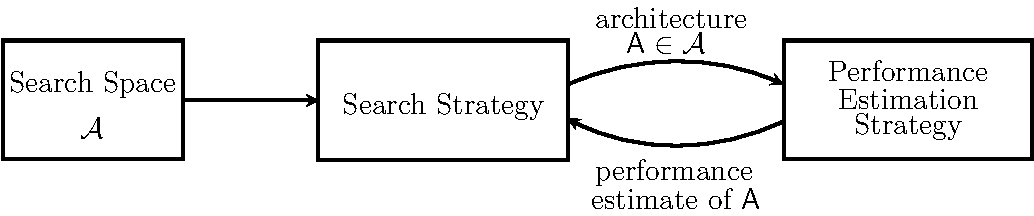
\includegraphics[width=0.8\linewidth]{figures/2_theory/nas_example.pdf}
    \caption[Ejemplo abstracto de los métodos de búsqueda de arquitectura neuronal]{Ejemplo abstracto de los métodos de búsqueda de arquitectura neuronal. Una estrategia de búsqueda (\textit{Search Strategy}) selecciona una arquitectura A dentro de un espacio de búsqueda predefinido (\textit{Search Space}) $\mathcal{A}$. Esta arquitectura es evaluada por una estrategia de estimación de rendimiento (\textit{Performance Estimation Strategy}), la cual devuelve el rendimiento estimado de A a la estrategia de búsqueda para generar una nueva arquitectura A para la siguiente iteración. Esto se realiza hasta que se llega a un criterio de parada predefinido. Figura tomada de \cite{elsken_neural_2018}.}

    \label{nas_example}
\end{figure}

La búsqueda de arquitectura neuronal (\textit{Neural Architecture Search}, NAS) \cite{zoph_neural_2017} pretende automatizar la generación de la estructura de una red neuronal. A diferencia de obtener una estructura por medio de conocimiento experto, se utilizan algoritmos para explorar e identificar la mejor arquitectura de red neuronal para una tarea específica. Este enfoque automatizado ayuda a optimizar el rendimiento, la velocidad y la eficacia \cite{ultralytics_busqueda_nas}. Motivo por el cual se está aplicando a este proyecto, y adicionalmente, porque no existen modelos preentrenados que se pudieran utilizar como una base.

El enfoque consiste en definir un espacio de búsqueda de posibles arquitecturas de red, establecer una estrategia para explorar este espacio y evaluar el rendimiento de cada arquitectura. Este proceso iterativo permite a NAS descubrir arquitecturas muy eficaces para tareas específicas que podrían no ser diseñadas intuitivamente por los humanos, y que a menudo igualan o superan las mismas tanto en exactitud como en uso de recursos y tamaño \cite{poyser_neural_2024}.

Si bien existen actualmente una gran cantidad de algoritmos NAS, estos se pueden clasificar en distintos grupos dependiendo de la estrategia utilizada para la exploración del espacio de búsqueda y estrategias de estimación de rendimiento \cite{elsken_neural_2018, baymurzina_review_2022, white_neural_2023}.

\subsection{Estrategías de búsqueda}
\subsubsection{Por métodos evolutivos}
Los métodos evolutivos o de \textit{neuroevolution} hacen uso de algoritmos evolutivos para la generación de la estructura de la red. La idea principal es la de ir modificando iterativamente la arquitectura por medio de una población de redes candidatas por el uso de operadores de cruce y mutación para incrementar su valor de evaluación o \textit{fitness}, en cada siguiente iteración se van cruzando las redes con el mejor \textit{fitness} para obtener descendientes hasta que se obtenga un valor deseado de \textit{fitness} o se llegue a un criterio de para definido. Notablemente, la función de optimización no tiene por qué ser diferenciable, por lo que resultan particularmente útiles para optimización multi objetivo. 

Este método ha demostrado obtener redes con la misma efectividad que las obtenidas por humanos, pero esto viene con el conocido alto coste computacional que requieren los algoritmos evolutivos. Adicionalmente existen los costos computacionales de entrenar desde cero cada integrante de la población por cada iteración para determinar su \textit{fitness}.

\subsubsection{Por optimización bayesiana}
La optimización bayesiana es un método para encontrar la mejor arquitectura de red utilizando un modelo probabilístico sustituto. Este modelo predice el rendimiento de distintas arquitecturas y se actualiza iterativamente a medida que se recopilan nuevos datos. Para decidir qué arquitecturas probar, se usa una función de adquisición, que equilibra la exploración (probar opciones nuevas) y la explotación (refinar las mejores opciones encontradas). Una vez seleccionada una arquitectura prometedora, se evalúa su rendimiento real y se incorpora esta información en el modelo. Este proceso se repite hasta alcanzar un criterio de parada definido.

Este método es muy popular en NAS debido a que, en comparación con otros métodos, obtiene arquitecturas buenas en pocas iteraciones y es capaz de soportar espacios de búsqueda complejos, aunque está limitada en escalabilidad y en la paralelización de la búsqueda.

\subsubsection{Por aprendizaje por refuerzo}
El método de aprendizaje por refuerzo (\textit{Reinforcement Learning}, RL) intenta mejorar la búsqueda en el espacio de soluciones utilizando un modelo controlador conocido como un \say{agente} que realiza una \say{acción} muestreando una arquitectura y recibe una \say{recompensa} que es alguna métrica de validación de la red neuronal, como por ejemplo el \textit{accuracy} de la misma. En este paradigma, el agente iterativamente aprende a generar la arquitectura que genere las mejores recompensas basándose en algoritmos de RL basados en políticas o en valores.

Este método se ha demostrado capaz de obtener redes con las mismas capacidades que las diseñadas a mano, con el mayor cuello de botella siendo la necesidad de reentrenar cada modelo para la siguiente iteración, aunque se han desarrollado variantes que permiten modificar una red parcialmente entrenada para ahorrar tiempo de cómputo.

\subsubsection{Por pesos compartidos}
Esta familia de métodos surge por los costos computacionales producidos por la necesidad de reentrenar cada red candidata desde cero. La solución propuesta permite que pesos de las neuronas estén compartidos entre diferentes redes.

Se puede realizar por el uso de una SuperRed (\textit{SuperNet}), donde un agente LSTM selecciona una subred para ser entrenada como una solución candidata al problema. De  esta forma las neuronas que son comunes para las distintas subredes van actualizándose en cada entrenamiento al mismo tiempo que el agente LSTM va aprendiendo qué subredes son las mejores para el problema. Si bien reduce substancialmente el tiempo de cómputo, poseen alto uso de memoria y necesitan ser cuidadosamente tuneadas, de lo contrario los pesos pueden interferirse entre sí provocando un colapso en su desempeño.

Otro método, denominado Búsqueda de Arquitectura Diferenciable (\textit{Differentiable Architecture Search}), en vez de tratar el espacio de búsqueda como algo discreto, se relaja para volverlo continuo representando las operaciones candidatas (por ejemplo: convoluciones, \textit{pooling} y saltos en las conexiones) como sumas ponderadas, permitiendo así hacer uso del \textit{backpropagation} para optimizar tanto los pesos de la red neuronal como la arquitectura misma. Reducen el tiempo de cómputo en comparación con otros métodos, pero de igual forma poseen un alto uso de memoria y son susceptibles a converger en operaciones demasiado simples.

\subsubsection{Por búsqueda aleatoria}
Este método es el más básico e ingenuo de los utilizados, se trata de seleccionar arquitecturas al azar de las posibilidades del espacio de búsqueda y quedarse con la que obtenga la mejor puntuación en la métrica seleccionada. Aunque se trate de un concepto bastante sencillo y que por lo general estos métodos se utilizan como bases para comparar los métodos anteriormente mencionados, se pueden obtener muy buenas arquitecturas si se ha diseñado el espacio de búsqueda correctamente.

\subsection{Espacios de búsqueda}
Hay que tomar en cuenta que las estrategias de búsqueda son independientes del espacio de búsqueda, la elección este espacio puede afectar drásticamente el desempeño de la red resultante, representa un importante compromiso entre el sesgo humano y la eficiencia de la búsqueda: si el tamaño del espacio de búsqueda es pequeño e incluye muchas decisiones seleccionadas manualmente, los algoritmos NAS tendrán más facilidad para encontrar una arquitectura de alto rendimiento. Por otro lado, si el espacio de búsqueda es grande y contiene bloques de construcción más primitivos, un algoritmo NAS necesitará ejecutarse durante más tiempo, pero existe la posibilidad de descubrir arquitecturas novedosas \cite{white_neural_2023}.

\subsubsection{Espacios de búsqueda basados en cadenas}
Los espacios de búsqueda basados en cadenas, como el nombre sugiere, tienen una topología sencilla: encadenar capas de operaciones para generar la arquitectura de la red. Son conceptualmente simples, lo cual los hacen fáciles de diseñar e implementar. También permiten que se encuentren con facilidad arquitecturas eficaces, pero por tener una topología tan sencilla es menos probable que se obtengan diseños de arquitecturas verdaderamente novedosas.

\subsubsection{Espacios de búsqueda basados en celdas}
Los espacios de búsqueda basados en celdas toma inspiración en el hecho que la mayoría de las arquitecturas del estado del arte para CNNs consisten en patrones repetidos múltiples veces, como por ejemplo, los bloques residuales en la familia de redes ResNets. Por lo tanto, en vez de intentar generar toda la red desde cero, se enfoca en buscar \say{celdas} relativamente pequeñas y apilarlas en secuencia para formar la arquitectura de la red. Cabe destacar que la forma de la red a gran escala se encuentra predefinida, pero cada bloque se puede componer de diferentes \say{celdas}. Son muy populares y pueden obtenerse con rapidez, pero como la macroestructura se encuentra ya fija, no permiten mucha expresividad y variación de las arquitecturas que se obtienen.

\subsubsection{Espacios de búsqueda jerárquicos}
A diferencia de los otros tipos de espacios de búsqueda, en lo que todo el diseño de la arquitectura es \say{plano} o diseñado en una sola capa, los espacios de búsqueda jerárquicos poseen múltiples niveles en los que se va definiendo la estructura de la red desde los parámetros más generales hasta los más específicos. Son extremadamente expresivos, permiten obtener redes complejas y diversas, además de que al tener la jerarquía se hace más efectivo la búsqueda del espacio lo que lo hace más eficiente también. Por otro lado, son bastante más complicados de diseñar e implementar.

\subsection{Estrategias de estimación de rendimiento}
Las estrategias de búsqueda discutidas anteriormente tienen como objetivo obtener una arquitectura neuronal que maximice algún criterio de rendimiento, como puede ser la \textit{accuracy} sobre datos no previamente observados. Para guiar este proceso de búsqueda, es necesario estimar el rendimiento de cada arquitectura candidata.

La forma más directa de hacerlo consiste en entrenar completamente la arquitectura y evaluar su rendimiento sobre un conjunto de datos de validación. Sin embargo, esta estrategia no resulta escalable en la práctica, especialmente cuando el espacio de búsqueda es amplio o las arquitecturas son complejas, ya que cada entrenamiento completo puede requerir un alto coste computacional.

Por ello, se han propuesto diversas alternativas que permiten acelerar la estimación del rendimiento sin necesidad de realizar un entrenamiento completo. Estas técnicas buscan aproximar el comportamiento final del modelo de forma más eficiente, reduciendo considerablemente el tiempo requerido por cada evaluación durante la búsqueda.

\subsubsection{Extrapolación de la curva de aprendizaje}
Esta técnica busca predecir el rendimiento final de una arquitectura neuronal a partir de un entrenamiento parcial, mediante la extrapolación de su curva de aprendizaje. Dicha curva está compuesta por los valores de rendimiento obtenidos en el conjunto de validación a lo largo de las primeras épocas de entrenamiento. La idea consiste en ajustar un modelo paramétrico a esta curva parcial con el objetivo de estimar cómo evolucionará el rendimiento en las siguientes épocas, evitando así la necesidad de completar el entrenamiento completo de cada arquitectura. Naturalmente su principal desventaja es que la curva predicha se desvíe del verdadero rendimiento que podría obtener el modelo.

\subsubsection{\textit{Proxies} sin coste}

Los denominados \textit{proxies} sin coste (\textit{Zero-Cost Proxies}) constituyen una familia de técnicas para la estimación rápida del rendimiento de arquitecturas neuronales. Su principio consiste en calcular métricas simples (por ejemplo, una única pasada de propagación hacia adelante y hacia atrás sobre un minilote de datos) para asignar una puntuación a cada arquitectura. La hipótesis subyacente es que dichas puntuaciones presentan una correlación con el rendimiento final real de las arquitecturas, permitiendo así identificar candidatos prometedores sin necesidad de entrenamiento completo. Se les considera \say{sin coste} porque su tiempo de cómputo es significativamente menor que el requerido por otras estrategias de evaluación. No obstante, su principal limitación radica en su escasa precisión al explorar espacios de búsqueda amplios, mostrando además una tendencia a favorecer arquitecturas de mayor tamaño o con mayor densidad de canales.

\subsubsection{Predicciones de baja fidelidad}
Una alternativa al entrenamiento completo de las arquitecturas consiste en realizar predicciones de bajo coste computacional mediante técnicas de baja fidelidad. Estas incluyen entrenar las arquitecturas durante un número reducido de épocas, emplear subconjuntos más pequeños del conjunto de datos, utilizar versiones degradadas de los datos (por ejemplo, imágenes de menor resolución) o bien simplificar la arquitectura evaluada, reduciendo el número de filtros por capa o el número de bloques estructurales. Aunque estas estrategias reducen significativamente el coste computacional, introducen sesgos que tienden a subestimar el rendimiento final del modelo. Para mitigar este efecto, es habitual que la estrategia de búsqueda utilice sistemas de ranking en lugar de valores absolutos, siempre que las posiciones relativas entre arquitecturas se mantengan consistentes. No obstante, si las simplificaciones aplicadas son demasiado extremas, estas relaciones pueden distorsionarse, por lo que se recomienda incrementar gradualmente la fidelidad de las predicciones conforme se refina el proceso de búsqueda.

\section{Representaciones 3D en \textit{Deep Learning}}
\label{section2:3dreps}
Actualmente, no existe un consenso claro en la literatura sobre la forma óptima de representar datos tridimensionales en el ámbito del DL, principalmente debido al desafío de adaptar las CNNs, originalmente diseñadas para trabajar con datos 2D regulares como las imágenes, a la naturaleza irregular de los datos en 3D.

A pesar de que la investigación en este campo es relativamente reciente, la creación del concurso anual 3D Shape Retrieval Challenge (SHREC) \cite{noauthor_shrec_nodate, noauthor_3dor2024_nodate}, centrado en evaluar múltiples tareas asociadas al análisis de datos 3D, ha incentivado la formulación de nuevas estrategias de representación orientadas a su procesamiento mediante técnicas de DL. 

En la literatura, se han identificado cinco principales categorías de representaciones tridimensionales en la tarea de clasificación: datos en bruto, sólidos, superficies, estructuras de alto nivel y datos de múltiples vistas (véase Figura \ref{fig:3dTaxonomy}). Esta clasificación fue propuesta inicialmente por Ahmed et al. \cite{ahmed_survey_2019} y posteriormente ampliada por Gezawa et al. \cite{gezawa_review_2020} y Muzahid et al. \cite{muzahid_deep_2024}.

\begin{figure}[h]
    \centering
    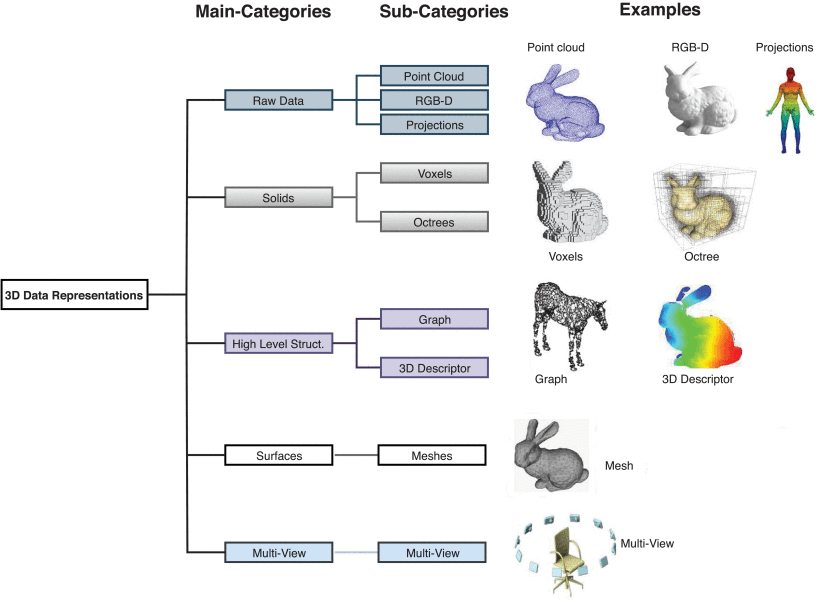
\includegraphics[width=\linewidth]{figures/2_theory/3Dtaxonomy.png}
    \caption[Taxonomía de las representaciones 3D para Deep Learning]{Taxonomía de las diferentes técnicas actuales en DL utilizadas para representar datos tridimensionales identificadas por \cite{gezawa_review_2020}}
    \label{fig:3dTaxonomy}
\end{figure}

\subsection{Datos en bruto}
Los datos en bruto corresponden a aquellos que pueden obtenerse mediante diferentes técnicas de escaneo, como cámaras de profundidad (por ejemplo, Microsoft Kinect o Intel RealSense) o escáneres basados en luz estructurada.

\subsubsection{Nube de Puntos}
En un espacio tridimensional, una nube de puntos se define como una colección de puntos discretos caracterizados por sus coordenadas $X$, $Y$ y $Z$. Cada coordenada especifica la posición de un punto dentro de un sistema cartesiano, aunque también pueden emplearse otros sistemas de referencia. La densidad y la distribución de los puntos permiten inferir la forma, estructura y características del objeto o entorno representado.

Se trata de una representación ampliamente utilizada debido a su simplicidad y a la facilidad con la que puede obtenerse mediante cámaras de profundidad o técnicas de fotogrametría LiDAR. No obstante, presenta limitaciones importantes: al estar compuesta únicamente por puntos, carece de un orden canónico y de información explícita sobre la conectividad entre ellos, lo que genera ambigüedades en la reconstrucción de las superficies. Se pueden tener también posibles incompletitudes y ruido en los datos u otras limitaciones por las condiciones del entorno durante el proceso de adquisición.

\subsubsection{Datos RGB-D}
Los datos RGB-D constituyen una representación 2.5D en la que se combina la información cromática de una imagen convencional en color (RGB) con un mapa de profundidad (\textit{Depth}, D) de la escena. Este tipo de representación se ha vuelto muy popular debido a la simplicidad con la que puede capturar tanto la apariencia superficial como cierta información geométrica de una escena, así como por el bajo coste y amplia disponibilidad de cámaras de profundidad.

No obstante, esta representación presenta limitaciones notables. En primer lugar, la información obtenida es parcial, ya que se captura únicamente desde el punto de vista de la cámara, lo que ocasiona oclusiones y pérdida de datos en regiones no visibles. Además, los sensores poseen un rango limitado de precisión en la medición de la profundidad, lo que afecta la calidad de la geometría recuperada, especialmente en objetos pequeños o en superficies reflectantes y translúcidas. Asimismo, la fiabilidad del mapa de profundidad depende en gran medida de las condiciones de iluminación y del entorno de captura, pudiendo introducir ruido, o artefactos indeseados.

\subsubsection{Proyecciones}
La representación mediante proyecciones consiste en transformar datos tridimensionales en superficies bidimensionales, con el objetivo de poder aplicar directamente los métodos de DL convencionales diseñados para imágenes 2D. Entre las técnicas más comunes se encuentran las proyecciones esféricas y cilíndricas, que permiten mapear la superficie de un objeto 3D sobre una imagen 2D de manera continua e invariante a rotaciones alrededor de un eje principal de proyección. En muchos enfoques se utilizan múltiples proyecciones desde diferentes ángulos, con el fin de capturar mayor información de la geometría del objeto y reducir las pérdidas asociadas a una sola vista.

Sin embargo, este enfoque presenta limitaciones importantes. En primer lugar, al proyectar la información 3D sobre un plano 2D se produce una pérdida intrínseca de información geométrica, lo que afecta a la precisión en la reconstrucción de detalles finos. Además, en objetos con superficies complejas o con un alto grado de oclusiones, las proyecciones pueden solapar o esconder partes relevantes de la geometría, generando regiones incompletas o distorsionadas.

\subsection{Sólidos}
Las representaciones de sólidos en modelos tridimensionales se centran en describir el espacio ocupado por un objeto en tres dimensiones, diferenciando de manera explícita entre regiones ocupadas y vacías. Estas representaciones permiten capturar también la estructura interna y la ocupación volumétrica del objeto, lo que proporciona una descripción más completa de su geometría.

\subsubsection{Vóxeles}
Los vóxeles consisten en una discretización del espacio 3D mediante una cuadrícula regular en la que cada celda (o vóxel, análogo tridimensional del píxel) indica si corresponde a una región ocupada por el objeto o bien a un espacio vacío. Además de la mera ocupación, los vóxeles pueden enriquecerse con información adicional, como la distinción entre regiones visibles, ocluidas o autoocluídas, o la codificación de propiedades físicas y geométricas derivadas del punto de vista. Debido a su estructura regular, los vóxeles facilitan la aplicación de técnicas de DL desarrolladas originalmente para datos 2D.

No obstante, esta representación presenta desventajas significativas. La principal es su alto costo computacional y de memoria, ya que la complejidad crece de manera cúbica con la resolución. Por ejemplo, duplicar la resolución de la cuadrícula implica multiplicar por ocho los requisitos de almacenamiento y cómputo. Esto limita el uso de vóxeles en aplicaciones que demandan un alto nivel de detalle geométrico.

\subsubsection{Árbol octal}
El árbol octal u \textit{octree} es una extensión de la representación de vóxeles que introduce una subdivisión jerárquica del espacio. En lugar de emplear una cuadrícula regular con resolución fija, el espacio tridimensional se divide de manera recursiva en ocho subceldas (hijos) cada vez que una región requiere mayor nivel de detalle. De esta forma, se obtiene una estructura de datos jerárquica que permite representar zonas complejas con alta resolución, mientras que las regiones homogéneas o vacías se representan con celdas más grandes, reduciendo significativamente el coste de almacenamiento y procesamiento. Sin embargo, presentan limitaciones: la representación de superficies curvas o muy suaves puede no ser suficientemente precisa, ya que la discretización sigue estando basada en cubos. Asimismo, el proceso de construcción y gestión de la estructura jerárquica implica una complejidad adicional en comparación con la voxelización directa.

\subsection{Estructuras de alto nivel}
Las estructuras de alto nivel consisten en representaciones concisas y abstractas de un objeto 3D que buscan capturar sus características más relevantes, en lugar de describirlo en todo su detalle geométrico. Este tipo de representaciones permiten reducir la complejidad de los datos y, al mismo tiempo, resaltar las propiedades discriminativas que hacen que un objeto pertenezca a una categoría específica.

\subsubsection{Descriptor 3D}
Los descriptores 3D constituyen un método tradicional ampliamente utilizado, generalmente en combinación con algoritmos de ML clásico más que con técnicas de DL. Se trata de representaciones diseñadas manualmente o \textit{handcrafted}, construidas a partir del conocimiento experto. Existen dos enfoques principales: los métodos globales, que caracterizan el objeto completo mediante un único vector de características capaz de capturar su forma general y apariencia global (por ejemplo: \textit{Shape Distribution}, ESF). Y los métodos locales, que extraen información de regiones específicas de la superficie, describiendo la geometría en torno a puntos clave (por ejemplo: \textit{Spin Images}, SHOT).

Entre sus ventajas destacan una representación concisa y la facilidad de procesamiento, lo que los hace especialmente útiles en tareas de comparación, análisis y recuperación de formas tridimensionales, en particular en contextos no supervisados. Sin embargo, presentan limitaciones notables: requieren un alto coste computacional en su extracción, pueden ser sensibles al ruido, oclusiones y variaciones de escala, y tienden a perder información fina en escenarios supervisados.

\subsubsection{Grafos}
La representación mediante grafos describe un objeto 3D conectando las diferentes partes de su superficie en una estructura discreta, donde los nodos representan los vértices y los arcos las conexiones entre ellos. Este enfoque permite modelar de forma explícita la conectividad local de la geometría, lo que facilita la aplicación de algoritmos eficientes de teoría de grafos para el análisis de la forma.

Entre sus ventajas destaca la flexibilidad para capturar relaciones estructurales y la posibilidad de aplicar técnicas avanzadas como las redes neuronales sobre grafos. Sin embargo, presentan limitaciones importantes: la representación de propiedades topológicas globales (como la presencia de agujeros, túneles o cavidades) resulta compleja, y el uso de grafos altamente densos plantea problemas de escalabilidad computacional al trabajar con datos de alta resolución.

\subsection{Superficies}
Este tipo de representación describe la envolvente externa de un objeto tridimensional, delimitando la región que separa el espacio interior del exterior mediante un conjunto de polígonos. Las superficies presentan la ventaja de ser geométricamente intuitivas, eficientes de visualizar y relativamente fáciles de procesar, ya que la mayoría pueden aproximarse a partir de combinaciones de ecuaciones lineales. Existen múltiples métodos para la representación superficial, entre los que destacan las superficies paramétricas, las implícitas y las basadas en subdivisiones. Sin embargo, la representación más popular y ampliamente utilizada, tanto en informática gráfica como en DL, es la malla poligonal, particularmente la malla triangular.

\subsubsection{Malla 3D}
Las mallas 3D están formadas por una combinación de vértices, aristas y caras. Cada vértice tiene asociada una lista de conectividad que indica cómo se conectan entre sí, y esta lista puede interpretarse como el conjunto de aristas que, a su vez, describen las caras de la malla. En la práctica, la mayoría de las mallas utilizan triángulos como unidad básica debido a su simplicidad y estabilidad matemática, aunque también se pueden emplear cuadriláteros u otros polígonos.

La principal ventaja de las mallas 3D es su amplia adopción y relevancia en informática gráfica, tanto para almacenar descripciones de modelos 3D como para su visualización. No obstante, debido a su irregularidad y complejidad, el estudio de su aplicación en tareas de DL no se había abordado satisfactoriamente hasta tiempos recientes. Hoy en día, se trata de una de las áreas más novedosas, con modelos que han alcanzado resultados satisfactorios, aunque con un alto consumo de recursos computacionales.

\subsection{Múltiples vistas}
Esta representación consiste en modelar un objeto 3D mediante un conjunto de imágenes tomadas desde diferentes puntos de vista, utilizando técnicas tradicionales de gráficos por ordenador. Posteriormente, estas imágenes se emplean como entradas para una CNN convencional.

La principal ventaja de esta representación es que permite aprovechar todas las técnicas y métodos ya existentes para CNNs basadas en imágenes, lo que facilita la utilización de modelos de alta resolución. Sin embargo, su mayor desventaja radica en la dificultad de determinar el número adecuado de puntos de vista a utilizar, así como en la pérdida de información que ocurre cuando partes del modelo 3D se solapan entre sí y quedan ocultas desde ciertos ángulos. Además, esta representación no conserva las propiedades geométricas intrínsecas del modelo 3D, y el uso de múltiples vistas conlleva un alto costo computacional.